\problemname{Access Points}

A well-known programming contest is considering a new way to position its teams.
For the contest all $n$ teams have to be assigned some position $(x,y)$ in an infinitely-large gym hall.
To keep a good overview of the teams the following strategy is chosen:

All teams have been assigned a unique integer ID in the range $[1,n]$.
Any two teams with IDs $i$ and $j$, where $i<j$, must be placed at positions $(x_i,y_i)$, $(x_j,y_j)$, such that $x_i \le x_j$ and $y_i \le y_j$.

Unfortunately, someone already assigned the (fixed) internet access point for each team.
The access points are quite big and only have one port, so access points for different teams are located at different positions.
Every team must be connected to its designated access point by a direct UTP cable.
The cost of a UTP cable of length $\ell$ is $\ell^2$.

Find a placement for all teams, such that their respective order along both axes is maintained and the total cost of the required UTP cables is minimised.
As the judges are not too worried about privacy, they are fine with two (or more) teams being placed at the exact same location or being arbitrarily close together.  See Figure~\ref{fig:contest} for an example.

\begin{figure}[h!]
  \centering
  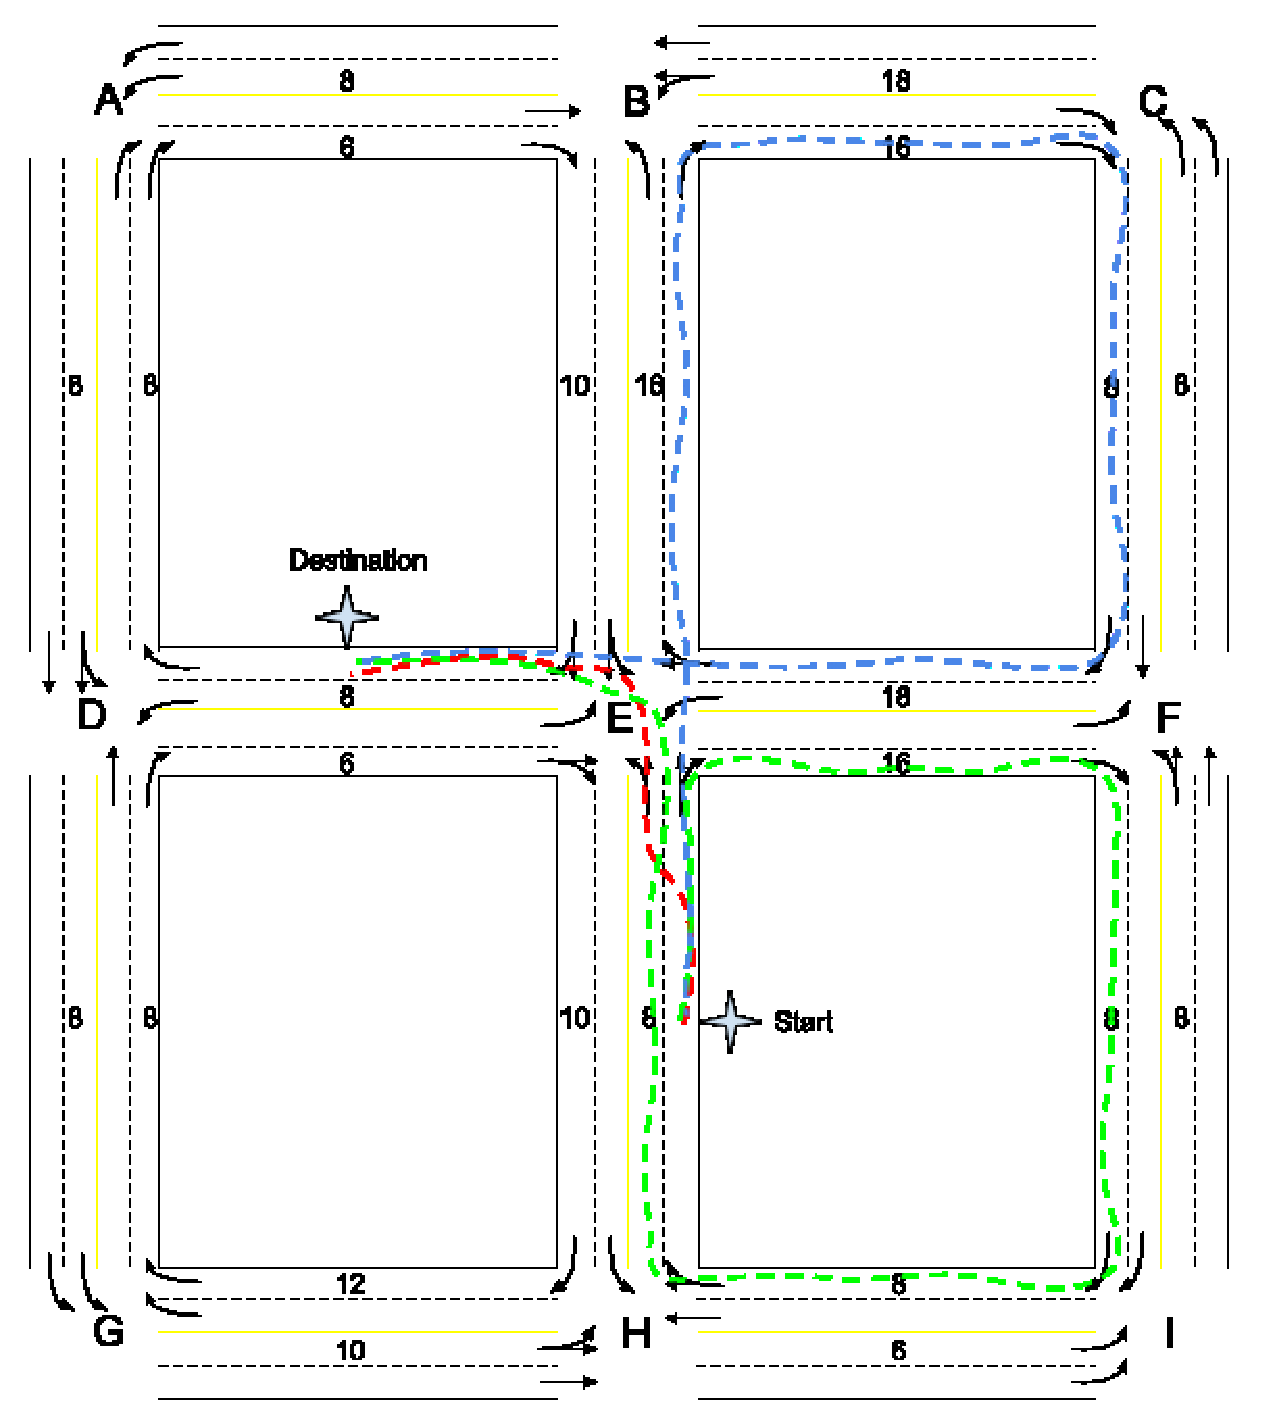
\includegraphics[width=0.63\textwidth]{figure}
  \caption{Illustration of an optimal placement for Sample Input 1. Team placement (boxes), access points (circles), and required UTP cables (dashed).}
  \label{fig:contest}
\end{figure}

\section*{Input}

The input consists of:
\begin{itemize}
	\item One line with one integer $n$ ($1 \le n \le 10^5$), the number of teams.
	\item $n$ lines, the $i$th of which contains two integers $s_i$, $t_i$ ($1 \le s_i,t_i \le 10^6$), the location of the internet access point of team $i$.
\end{itemize}
No two access points are at the same position.

\section*{Output}
Output the minimum total cost of all UTP cables required to connect the teams to their access points in an optimal legal layout.

Your answer should have an absolute or relative error of at most $10^{-6}$.
